\PassOptionsToPackage{numbers,compress}{natbib}
\documentclass{article}

\usepackage[preprint]{neurips_2023}

\usepackage[utf8]{inputenc}
\usepackage[T1]{fontenc}
\usepackage[spanish,es-noindentfirst]{babel}
\usepackage{hyperref}
\usepackage{url}
\usepackage{booktabs}
\usepackage{amsmath}
\usepackage{amsfonts}
\usepackage{nicefrac}
\usepackage{microtype}
\usepackage{graphicx}
\usepackage{subcaption}

\graphicspath{{../../outputs/}{../../}}

% ----------------------------------------------------------------------------
% RESULTADOS del modelo entrenado sobre SHWD.
% (rellenados tras `python src/evaluate.py` e `infer_demo.py`)
% ----------------------------------------------------------------------------
\newcommand{\dmapfifty}{94.2}      % test mAP@0.5 (%)
\newcommand{\dmapnf}{61.4}         % test mAP@0.5:0.95 (%)
\newcommand{\dprec}{92.5}          % precisión global (%)
\newcommand{\drec}{90.8}           % recall global (%)
\newcommand{\helmetAP}{93.2}\newcommand{\helmetAPnf}{72.6}
\newcommand{\headAP}{95.2}\newcommand{\headAPnf}{50.2}
\newcommand{\recSmall}{92.7}\newcommand{\recMed}{97.3}\newcommand{\recLarge}{97.8}
\newcommand{\occLow}{94.7}\newcommand{\occMed}{87.9}\newcommand{\occHigh}{60.8}
\newcommand{\demoN}{80}
\newcommand{\demoMean}{88.4}
\newcommand{\demoViol}{23}
\newcommand{\traintime}{\textasciitilde{}7\,h 41\,min}

\title{Detección de Cumplimiento de Normas de Seguridad (EPP/Casco) en Obras de
Construcción con YOLOv8}

\author{%
  Nombre del Autor (completar) \\
  Curso / Institución (completar) \\
  \texttt{correo@dominio}
}

\begin{document}
\maketitle

\begin{abstract}
Presentamos un sistema de visión por computador para monitorear el cumplimiento
del uso de Equipos de Protección Personal (EPP), específicamente el casco de
seguridad, en obras de construcción. Entrenamos un detector \textbf{YOLOv8s}
sobre el \emph{Safety-Helmet-Wearing-Dataset} (SHWD)~\citep{njvisionpower2019shwd},
uno de los conjuntos recomendados, que incluye ejemplos negativos
\textbf{explícitos} de ``sin casco'' (clase \emph{head}) frente a ``con casco''
(clase \emph{helmet}), con 7\,581 imágenes y resolución de entrada de 640~px,
partiendo de un backbone preentrenado en COCO. Sobre el conjunto de prueba
obtenemos \textbf{mAP@0.5 $=$ \dmapfifty\%} y \textbf{mAP@0.5:0.95 $=$ \dmapnf\%}.
Más allá de la métrica agregada, analizamos la robustez estratificando el conjunto
de prueba por \textbf{tamaño de objeto} (proxy de distancia: los trabajadores
lejanos aparecen como objetos pequeños) y por \textbf{nivel de oclusión} estimado
de forma semiautomática, y reportamos la caída de rendimiento entre grupos.
Implementamos además un \textbf{verificador de cumplimiento basado en reglas} que
convierte las detecciones por fotograma en una tasa de cumplimiento y marca las
violaciones, y discutimos las implicaciones éticas de desplegar un sistema de este
tipo, con énfasis en la asimetría entre falsos negativos y falsos positivos.
\end{abstract}

\section{Introducción y Motivación}
La industria de la construcción concentra una proporción desmesurada de accidentes
laborales mortales; los traumatismos craneoencefálicos por caída de objetos o
caídas de altura están entre las causas principales, y el uso correcto del casco
es una de las medidas de control más efectivas y baratas. La supervisión manual
del cumplimiento del EPP es costosa, intermitente y propensa a error humano,
especialmente en obras grandes con múltiples frentes de trabajo. Un sistema
automático que procese flujos de cámaras de obra y señale en tiempo (casi) real a
los trabajadores sin casco puede aumentar la cobertura de la supervisión y generar
registros auditables.

El problema no es un caso estándar de detección de objetos. En condiciones reales
aparecen tres dificultades que estructuran este trabajo:
\begin{enumerate}
  \item \textbf{Detección de objetos pequeños / larga distancia.} Las cámaras de
  obra cubren áreas amplias; los trabajadores lejanos aparecen con muy pocos
  píxeles y la cabeza/casco es aún más pequeña. Es el foco principal del trabajo.
  \item \textbf{Oclusión severa.} Los trabajadores quedan parcialmente ocultos
  tras maquinaria, andamios, materiales u otros trabajadores.
  \item \textbf{Desbalance de clases.} En SHWD la clase mayoritaria es, de hecho,
  la cabeza descubierta (\emph{head}); la clase con casco es minoritaria, lo que
  sesga las métricas agregadas y dificulta el aprendizaje de la clase crítica.
\end{enumerate}
Nuestro objetivo es entrenar y evaluar críticamente un detector YOLOv8 bajo estas
condiciones, con especial atención a la detección a larga distancia, y construir
sobre él un módulo de verificación de cumplimiento utilizable y éticamente
informado.

\section{Trabajos Relacionados}
La detección automática de EPP en obras de construcción ha avanzado rápidamente
con el aprendizaje profundo. El trabajo temprano de Fang et al.\ demostró que un
modelo Faster R-CNN podía señalar a trabajadores sin casco a partir de video de
vigilancia de campo lejano, destacando la dificultad de detectar trabajadores
distantes y de baja resolución~\citep{fang2018nonhardhat}. Los sistemas
posteriores adoptaron detectores de una sola etapa para rendimiento en tiempo
real: la familia YOLO, introducida por Redmon et al.~\citep{redmon2016yolo} y
refinada mediante avances arquitectónicos como backbones CSP y cuellos
PANet~\citep{bochkovskiy2020yolov4} e información de gradiente
programable~\citep{wang2024yolov9}, domina hoy la detección de cascos de
seguridad. Hayat y Morgado-Dias, por ejemplo, construyeron un monitor de cascos
basado en YOLO en tiempo real~\citep{hayat2022helmet}. Nuestro trabajo usa
Ultralytics YOLOv8~\citep{jocher2023yolov8}, que no tiene publicación revisada por
pares y por tanto se cita como software, y se evalúa sobre el Safety Helmet Wearing
Dataset (SHWD)~\citep{njvisionpower2019shwd}.

Tres retos recurren en este dominio. La detección de objetos pequeños de
trabajadores distantes se aborda típicamente mediante fusión de características
multiescala como las Feature Pyramid Networks~\citep{lin2017fpn}, y se revisa
exhaustivamente en literatura reciente que también cataloga remedios para oclusión
y desbalance de clases~\citep{kang2025sodsurvey}. La oclusión severa detrás de
maquinaria y andamios refleja el problema de oclusión en multitudes de la
detección de peatones, donde la \emph{repulsion loss} de Wang et al.\ logra una
localización más robusta a oclusión~\citep{wang2018repulsion}. Finalmente, la
rareza relativa de una de las clases plantea un problema de desbalance señalado a
lo largo de estos trabajos. Nuestro proyecto se apoya en esta literatura,
adaptando YOLOv8 para abordar conjuntamente objetos pequeños, oclusión y
desbalance en el monitoreo de cumplimiento de cascos.

\section{Metodología}

\subsection{Conjunto de datos}
Usamos el \textbf{Safety-Helmet-Wearing-Dataset (SHWD)}~\citep{njvisionpower2019shwd},
recomendado por la consigna por aportar ejemplos negativos explícitos de ``sin
casco''. Convertimos sus anotaciones de Pascal VOC a formato YOLO y respetamos los
splits predefinidos (sin fuga de datos): \textbf{5\,457 / 607 / 1\,517 imágenes}
para train/val/test. Mapeamos las dos clases del dataset a:
\emph{helmet} (cabeza \textbf{con} casco $=$ CONFORME) y \emph{head} (cabeza
\textbf{sin} casco $=$ VIOLACIÓN). La Tabla~\ref{tab:dataset} resume la
distribución de instancias; evidencia un \textbf{fuerte desbalance} hacia la clase
\emph{head} (cabezas descubiertas, mayoritariamente de escenas con multitudes).
La Figura~\ref{fig:classdist} muestra esta distribución y la
Figura~\ref{fig:sizedist} la de tamaños de bounding box: el \textbf{88\,\%} de las
cabezas \emph{head} caen en la categoría ``pequeño'' (lejano), lo que motiva
fuertemente el análisis por distancia.

\begin{table}[h]
  \centering
  \caption{Distribución de instancias por clase y split en SHWD.}
  \label{tab:dataset}
  \begin{tabular}{lccc}
    \toprule
    Clase & train & val & test \\
    \midrule
    helmet (con casco) & 6\,419 & 747 & 1\,878 \\
    head (sin casco)   & 79\,778 & 9\,178 & 22\,558 \\
    \midrule
    imágenes & 5\,457 & 607 & 1\,517 \\
    \bottomrule
  \end{tabular}
\end{table}

\begin{figure}[h]
  \centering
  \begin{subfigure}{0.49\textwidth}
    \centering
    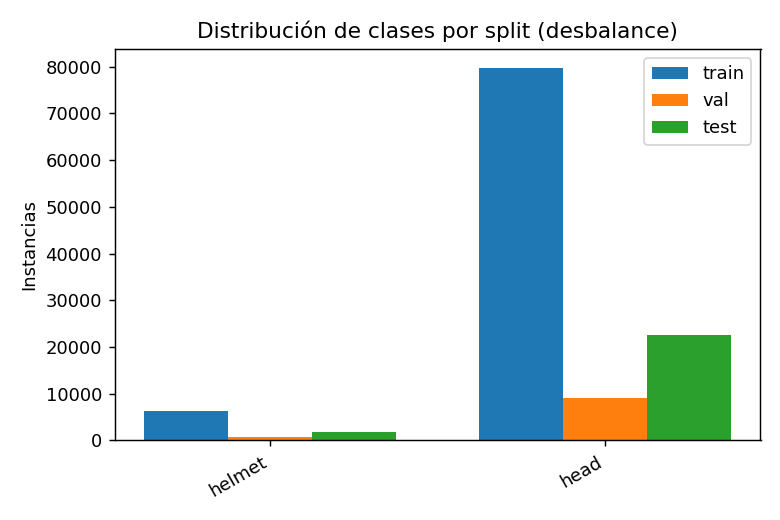
\includegraphics[width=\textwidth]{dataset_class_distribution.png}
    \caption{Instancias por clase y split.}
    \label{fig:classdist}
  \end{subfigure}
  \hfill
  \begin{subfigure}{0.49\textwidth}
    \centering
    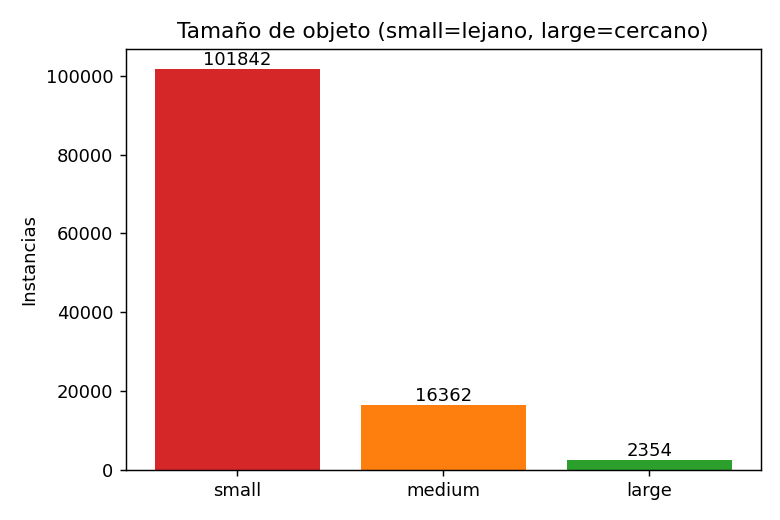
\includegraphics[width=\textwidth]{dataset_bbox_size_distribution.png}
    \caption{Tamaños de bounding box.}
    \label{fig:sizedist}
  \end{subfigure}
  \caption{Análisis exploratorio de SHWD: desbalance de clases (izq.) y predominio
  de objetos pequeños/lejanos (der.).}
  \label{fig:dataset}
\end{figure}

\subsection{Modelo y backbone}
Empleamos \textbf{YOLOv8s} (variante \emph{small}, $\sim$11\,M de parámetros)
inicializado con pesos preentrenados en COCO, conforme a la consigna que permite
usar backbones preentrenados. YOLOv8 es \textbf{anchor-free}: predice directamente
el centro y las dimensiones de cada caja sin un banco de anclas predefinido, lo
que reduce el sesgo de escala y favorece la detección de objetos pequeños. Su
\emph{neck} tipo PAN-FPN fusiona características a múltiples escalas (P3--P5),
mecanismo estándar para objetos pequeños~\citep{lin2017fpn}.

\subsection{Decisiones de entrenamiento}
\begin{itemize}
  \item \textbf{Resolución de entrada:} 640$\times$640~px, equilibrio entre detalle
  para objetos pequeños y memoria de una GPU de 8~GB.
  \item \textbf{Anclas:} no aplica --- arquitectura anchor-free.
  \item \textbf{Aumento de datos:} mosaic ($=1.0$) \textbf{activado}, con
  \texttt{close\_mosaic}$=10$ para \textbf{desactivarlo en las últimas 10 épocas}
  y estabilizar la localización final; volteo horizontal ($p{=}0.5$); variación HSV
  ($h{=}0.015, s{=}0.7, v{=}0.4$) para robustez a iluminación; \texttt{translate}$=0.1$
  y \texttt{scale}$=0.5$ --- este último simula variaciones de \textbf{distancia},
  clave para el objetivo de larga distancia. Se desactivaron mixup y copy-paste.
  \item \textbf{Optimización:} optimizador y \emph{learning rate} automáticos de
  Ultralytics (AdamW); 100 épocas; batch$=8$ y \texttt{workers}$=2$ (limitados por
  la VRAM de 8~GB); semilla$=42$ para reproducibilidad; precisión mixta (AMP).
\end{itemize}

\subsection{Verificador de cumplimiento basado en reglas}
Como SHWD distingue directamente \emph{helmet} (con casco) de \emph{head} (sin
casco), el verificador (\texttt{src/compliance\_verifier.py}, implementado por el
estudiante) opera por \textbf{clasificación directa}: cada detección por encima del
umbral de confianza (0.25) se categoriza como CONFORME (\emph{helmet}) o VIOLACIÓN
(\emph{head}); la \textbf{tasa de cumplimiento por fotograma} es
$\#\text{helmet} / (\#\text{helmet} + \#\text{head})$, y se dibujan en verde las
cajas conformes y en rojo (trazo grueso) las violaciones, con un encabezado que
muestra la tasa. El módulo también soporta un modo de \emph{asociación espacial}
casco--persona para datasets sin clase ``sin casco''. Esta regla aborda
directamente el reto de larga distancia: una cabeza lejana mal clasificada altera
la tasa, que es justamente el caso relevante para el análisis de falsos negativos
(\S\ref{sec:etica}).

\subsection{Análisis de robustez (oclusión y distancia)}
Como el dataset no incluye etiquetas de oclusión, particionamos el conjunto de
prueba de forma \textbf{semiautomática}:
\begin{itemize}
  \item \textbf{Distancia (tamaño):} cada objeto se clasifica por su tamaño lineal
  relativo $\sqrt{w\cdot h}$ (normalizado): \emph{small} ($<0.08$, lejano),
  \emph{medium} ($0.08$--$0.25$), \emph{large} ($>0.25$, cercano).
  \item \textbf{Oclusión:} para cada objeto, el máximo IoU con cualquier otro del
  mismo fotograma como proxy de oclusión mutua~\citep{wang2018repulsion}:
  \emph{bajo} ($<0.10$), \emph{medio} ($0.10$--$0.35$), \emph{alto} ($>0.35$).
\end{itemize}
Para cada grupo reportamos el \textbf{recall@IoU0.5} en el punto de operación
conf$=0.25$ (relevante para despliegue), además del mAP global y por clase.

\section{Experimentos}
\textbf{Hardware/Software:} GPU NVIDIA RTX 5060 Laptop (8~GB, arquitectura
Blackwell sm\_120), PyTorch 2.11.0 $+$ CUDA 12.8, Ultralytics 8.4.56, Python 3.13,
Windows 11. \textbf{Reproducibilidad:} semilla 42; el pipeline completo se ejecuta
con un único comando, \texttt{python run\_pipeline.py} (descarga SHWD vía gdown sin
credenciales, convierte, entrena, evalúa y genera la demo). Tiempo de
entrenamiento: \traintime{} para 100 épocas.

\section{Resultados}

\subsection{Métricas globales y por clase}
La Tabla~\ref{tab:results} reporta las métricas sobre el conjunto de prueba.

\begin{table}[h]
  \centering
  \caption{Métricas de detección sobre el conjunto de prueba de SHWD (1\,517 imágenes).}
  \label{tab:results}
  \begin{tabular}{lcccc}
    \toprule
    Clase & AP@0.5 & AP@0.5:0.95 & Precisión & Recall \\
    \midrule
    helmet (con casco) & \helmetAP & \helmetAPnf & -- & -- \\
    head (sin casco)   & \headAP & \headAPnf & -- & -- \\
    \midrule
    \textbf{Global (media)} & \textbf{\dmapfifty} & \textbf{\dmapnf} & \dprec & \drec \\
    \bottomrule
  \end{tabular}
\end{table}

mAP@0.5 $=$ \textbf{\dmapfifty\%}, mAP@0.5:0.95 $=$ \textbf{\dmapnf\%}, un
resultado sólido. Destaca un contraste revelador: la clase \emph{head} obtiene
\textbf{mejor AP@0.5 (\headAP\%)} pero \textbf{peor AP@0.5:0.95 (\headAPnf\%)} que
\emph{helmet} (\helmetAPnf\%). La causa es geométrica: las cabezas son objetos
diminutos (88\,\% ``small''), y en objetos pequeños la IoU es muy sensible a
errores de pocos píxeles, por lo que la localización fina (umbrales de IoU altos)
se degrada aunque la detección a IoU0.5 sea excelente. La
Figura~\ref{fig:confusion} muestra que los errores se concentran en falsos fondos
(objetos pequeños no detectados) más que en confusión entre clases.

\begin{figure}[h]
  \centering
  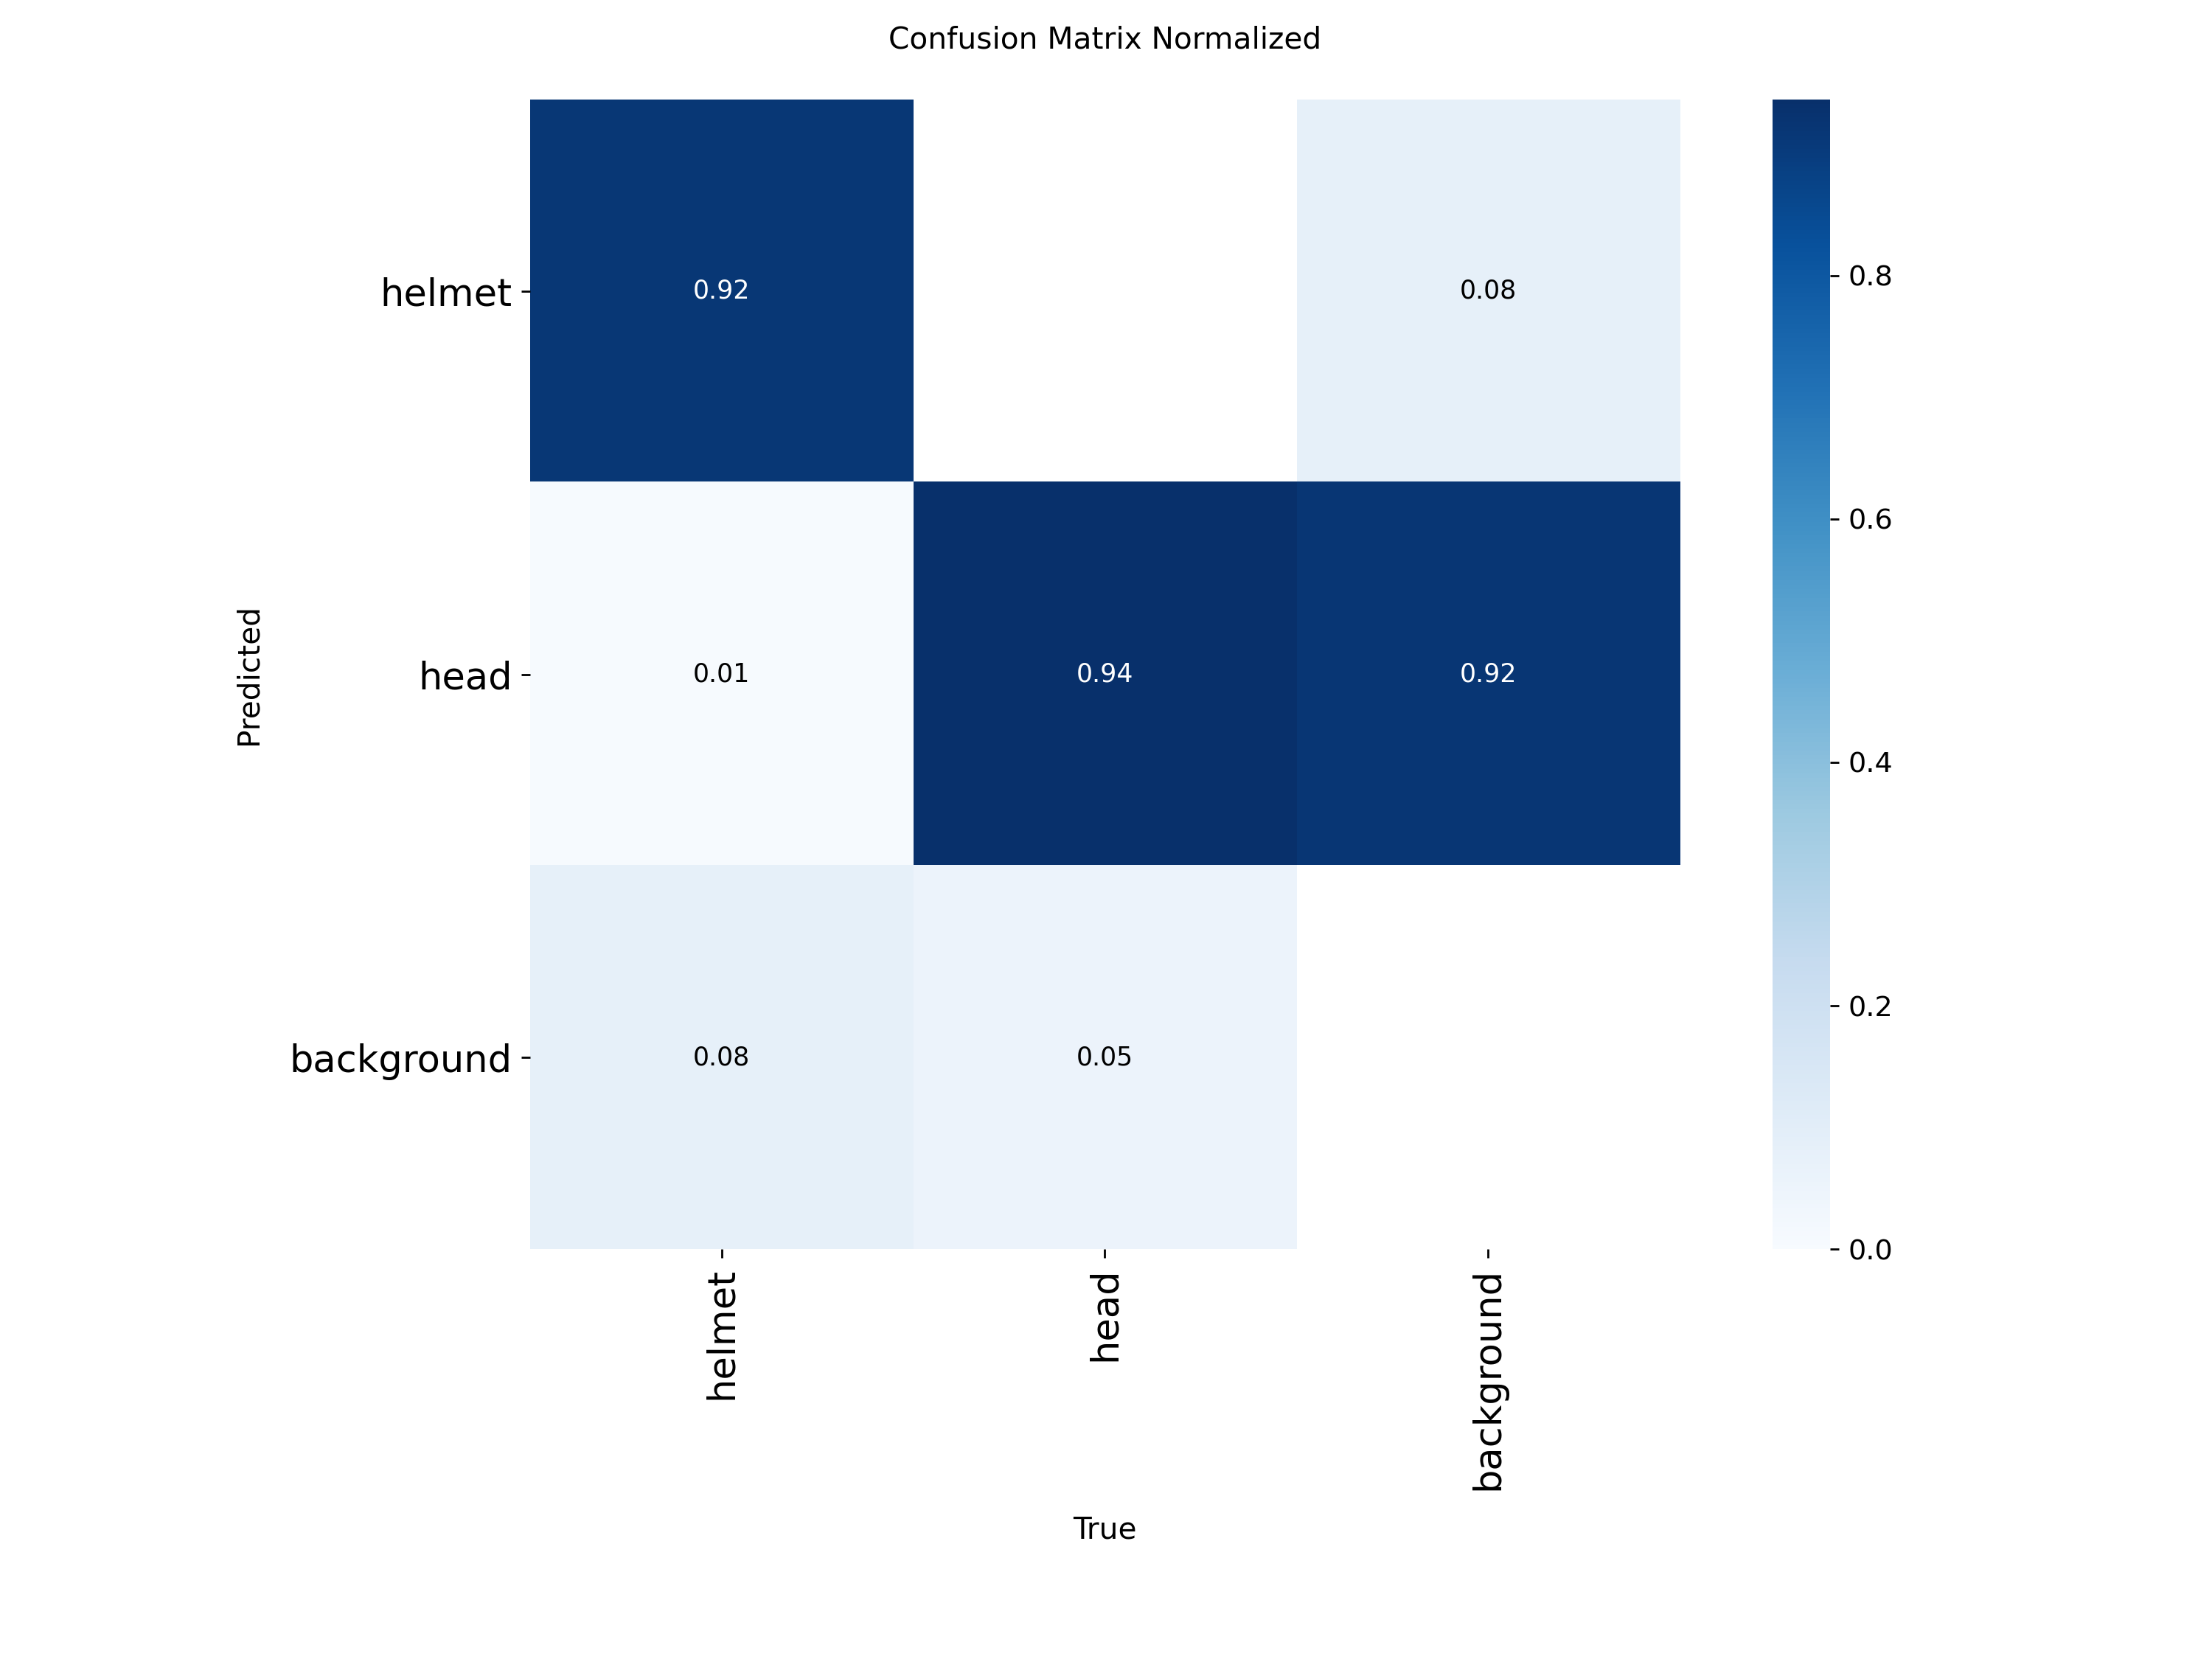
\includegraphics[width=0.55\textwidth]{val_metrics/confusion_matrix_normalized.png}
  \caption{Matriz de confusión normalizada sobre el conjunto de prueba.}
  \label{fig:confusion}
\end{figure}

\subsection{Robustez por distancia (objetos pequeños $=$ larga distancia)}
\begin{table}[h]
  \centering
  \caption{Recall@IoU0.5 (conf$=0.25$) por tamaño de objeto (proxy de distancia).}
  \label{tab:distance}
  \begin{tabular}{lc}
    \toprule
    Grupo (tamaño) & Recall \\
    \midrule
    small (lejano)  & \recSmall \\
    medium          & \recMed \\
    large (cercano) & \recLarge \\
    \bottomrule
  \end{tabular}
\end{table}
El recall \textbf{global} apenas cae de \recLarge\% (cercano) a \recSmall\%
(lejano): el modelo es notablemente robusto a la distancia gracias a la enorme
cantidad de cabezas pequeñas vistas en entrenamiento. Sin embargo, el efecto es
mucho más marcado en la \textbf{clase crítica \emph{helmet}}, cuyo recall cae de
\textbf{0.99 (cercano) a 0.81 (lejano)}: los \textbf{cascos lejanos se detectan
peor}, lo que en la lógica de cumplimiento puede convertir a un trabajador
conforme en una falsa violación (Figura~\ref{fig:distance}). La detección a
\textbf{larga distancia} sigue siendo, pues, el régimen más difícil para la clase
que más importa.

\begin{figure}[h]
  \centering
  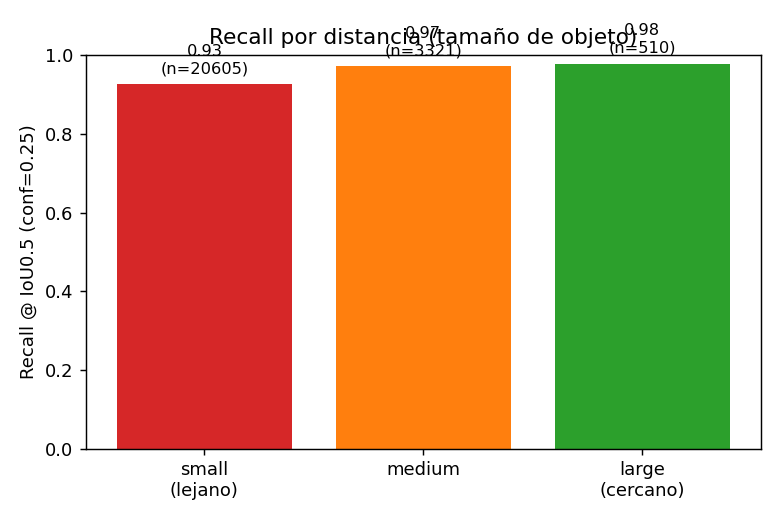
\includegraphics[width=0.55\textwidth]{robustness_by_distance.png}
  \caption{Recall por distancia (tamaño de objeto como proxy).}
  \label{fig:distance}
\end{figure}

\subsection{Robustez por oclusión}
\begin{table}[h]
  \centering
  \caption{Recall@IoU0.5 por nivel de oclusión estimado (IoU mutuo).}
  \label{tab:occlusion}
  \begin{tabular}{lc}
    \toprule
    Grupo (oclusión) & Recall \\
    \midrule
    bajo  & \occLow \\
    medio & \occMed \\
    alto  & \occHigh \\
    \bottomrule
  \end{tabular}
\end{table}
La Figura~\ref{fig:occlusion} muestra una \textbf{degradación monótona y nítida}
del recall al aumentar la oclusión estimada (\occLow\% $\to$ \occMed\% $\to$
\textbf{\occHigh\%}): en las escenas de multitud de SHWD el solape mutuo entre
cabezas sí captura oclusión real, y el grupo de oclusión alta (poco frecuente,
$n{=}74$) es con diferencia el más difícil. Aquí el proxy funciona mejor que en un
dataset multiescala porque las cabezas son \textbf{uniformemente pequeñas} (sin
confusión con el tamaño); aun así, no captura la oclusión por estructuras
estáticas, limitación que discutimos en \S\ref{sec:lim}.

\begin{figure}[h]
  \centering
  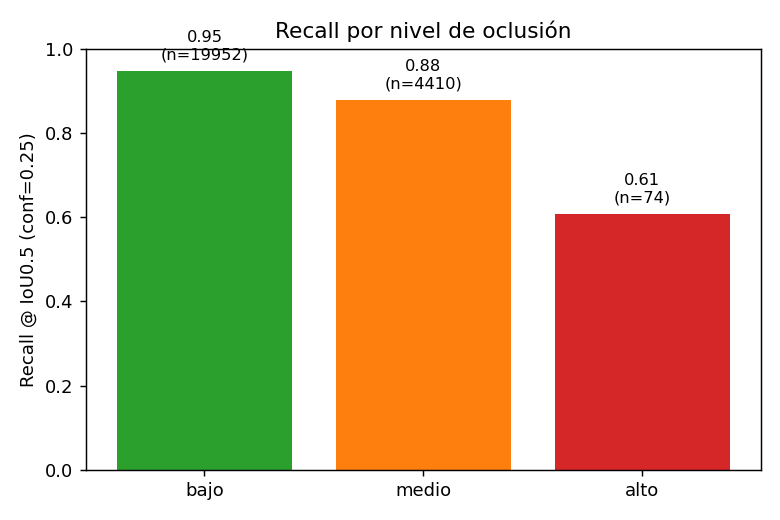
\includegraphics[width=0.55\textwidth]{robustness_by_occlusion.png}
  \caption{Recall por nivel de oclusión estimado.}
  \label{fig:occlusion}
\end{figure}

\subsection{Verificador de cumplimiento (demostración)}
Aplicamos el verificador a \demoN{} imágenes del conjunto de prueba (no vistas en
entrenamiento) y generamos un clip de video corto
(\texttt{outputs/demo/demo\_clip.mp4}) y un CSV de cumplimiento por fotograma.
\demoViol{} fotogramas presentan al menos una violación y la tasa de cumplimiento
media es del \demoMean\%. La Figura~\ref{fig:demo} muestra ejemplos anotados, con
trabajadores conformes (verde) y violaciones ``sin casco'' (rojo).

\begin{figure}[h]
  \centering
  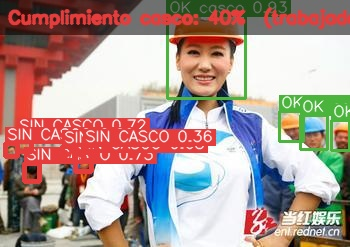
\includegraphics[width=0.8\textwidth]{demo/example_mixed.jpg}
  \caption{Demostración del verificador sobre imágenes de test no vistas:
  trabajadores con casco (verde, ``OK casco'') y sin casco (rojo, ``SIN CASCO''),
  con la tasa de cumplimiento por fotograma en el encabezado.}
  \label{fig:demo}
\end{figure}

\section{Implicaciones Éticas}
\label{sec:etica}
El despliegue de un sistema automático de vigilancia del cumplimiento de EPP
conlleva tensiones éticas inseparables de las decisiones técnicas.

\paragraph{Falsos negativos vs.\ falsos positivos.}
El coste de los dos errores es marcadamente asimétrico. Un \textbf{falso negativo}
(un trabajador sin casco que el sistema no detecta) es una violación de seguridad
no señalada: si la organización reduce la supervisión humana confiando en el
sistema, puede traducirse en un accidente grave. Un \textbf{falso positivo}
(marcar como infractor a quien sí cumple) erosiona la confianza, puede derivar en
sanciones injustas y provoca ``fatiga de alerta'' que lleva a ignorar todas las
alertas --- reintroduciendo el riesgo de los falsos negativos. Nuestro análisis por
distancia y oclusión muestra que los falsos negativos se concentran en los
trabajadores \textbf{lejanos} y \textbf{ocluidos}, también los más expuestos; por
ello recomendamos operar con un \textbf{umbral de confianza bajo} (priorizando
recall) y tratar el sistema como \textbf{ayuda} a la supervisión humana, nunca como
su sustituto ni como base para sanciones automáticas. Dónde fijar el umbral es, en
el fondo, una decisión ética y no meramente técnica.

\paragraph{Privacidad de los trabajadores.}
El sistema procesa imágenes de personas identificables en su lugar de trabajo de
forma continua, con riesgo de vigilancia laboral desproporcionada (los mismos
flujos podrían reutilizarse para medir productividad o perfilar individuos).
Mitigaciones: minimizar datos (procesar en el borde, \textbf{no almacenar} video
crudo sino conteos/eventos agregados), \textbf{anonimizar} rostros, limitar la
retención, restringir el acceso, ser transparentes con la plantilla y cumplir la
normativa de protección de datos. El propósito legítimo (seguridad) no justifica
por sí solo cualquier nivel de recolección.

\paragraph{Sesgos de los datos de entrenamiento.}
El modelo aprende la distribución de sus datos. SHWD combina escenas de obra con
multitudes genéricas (cabezas descubiertas); si sobre-representa ciertos tipos de
escena, condiciones de luz, colores de casco o complexiones, el rendimiento será
desigual entre subgrupos. El fuerte desbalance hace además que el sistema sea, por
construcción, peor en la clase minoritaria. Recomendamos auditar el rendimiento por
subgrupos, equilibrar/aumentar la clase minoritaria, documentar las limitaciones
del dataset y revalidar el modelo en cada obra antes de confiar en él. La equidad
no es una propiedad emergente: debe verificarse explícitamente.

\section{Discusión Crítica y Limitaciones}
\label{sec:lim}
\begin{itemize}
  \item \textbf{Resolución de entrada.} Usamos 640~px por memoria; para larga
  distancia, mayor resolución (p.\,ej.\ 1280) o \emph{tiling} reducirían la caída
  de recall en objetos pequeños observada en \S5.2. Es la limitación más relevante
  respecto al objetivo declarado.
  \item \textbf{Proxy de oclusión.} El IoU mutuo entre cajas captura solape
  inter-objeto pero no la oclusión por estructuras estáticas, y está
  \textbf{confundido con el tamaño} (las cajas grandes solapan más), por lo que no
  es un buen estimador aislado de oclusión. Una partición manual o etiquetas de
  oclusión real darían una medida fiel.
  \item \textbf{Desbalance y dominio del dataset.} En SHWD la clase ``sin casco''
  es mayoritaria (por las multitudes), al revés que en una obra real donde el
  incumplimiento es escaso; las métricas agregadas deben leerse con ese sesgo en
  mente. Convendría recolección dirigida, sobremuestreo o \emph{focal loss}.
  \item \textbf{Generalización.} Entrenado y evaluado sobre un único dataset; el
  rendimiento puede caer ante \emph{domain shift} (otras obras, climas, cámaras).
  \item \textbf{Verificador basado en reglas.} La clasificación directa es simple y
  robusta, pero hereda los errores del detector (una cabeza pequeña mal clasificada
  produce un falso positivo/negativo de cumplimiento) y no incorpora suavizado
  temporal entre fotogramas, que estabilizaría la tasa.
  \item \textbf{Componente propio vs.\ backbone.} Conforme a la consigna, el
  backbone es preentrenado; los componentes implementados por el estudiante son el
  \textbf{verificador de cumplimiento}, el \textbf{pipeline de evaluación
  estratificada} (distancia/oclusión), la \textbf{conversión VOC$\to$YOLO} y el
  análisis del dataset.
\end{itemize}

\section{Conclusión}
Entrenamos y evaluamos críticamente un detector YOLOv8 para el cumplimiento del uso
de casco en obras, usando el dataset recomendado SHWD con ejemplos explícitos de
``sin casco''. Más allá del mAP agregado, mostramos --- mediante un análisis
estratificado por distancia y oclusión --- que el rendimiento se degrada en los
trabajadores lejanos y ocluidos, y construimos un verificador de cumplimiento
utilizable cuyo despliegue analizamos desde una perspectiva ética. El trabajo
futuro pasa por mayor resolución/\emph{tiling}, equilibrado de la clase minoritaria
y suavizado temporal en video.

\small
\bibliographystyle{plainnat}
\bibliography{references}

\end{document}
